\documentclass{beamer}
\usepackage[utf8]{inputenc}
\usepackage{graphicx, epsfig}
\usepackage{amsmath,mathrsfs,amsfonts,amssymb}
\usepackage{floatflt}
\usepackage{epic,ecltree}
\usepackage{mathtext}
\usepackage{fancybox}
\usepackage{fancyhdr}
\usepackage{multirow}
\usepackage{enumerate}
\usepackage{epstopdf}
\usepackage{multicol}
\usepackage{algorithm}
\usepackage[noend]{algorithmic}
\usepackage{tikz}
\usepackage{blindtext}
\usepackage{multido}
\usetheme{default}%{Singapore}%{Warsaw}%{Warsaw}%{Darmstadt}
\usecolortheme{default}

\setbeamerfont{title}{size=\Huge}
\setbeamertemplate{footline}[frame number]{}

\setbeamertemplate{section in toc}[sections numbered]

\makeatletter
\newcommand\HUGE{\@setfontsize\Huge{35}{40}}
\makeatother    

\setbeamerfont{title}{size=\HUGE}
\beamertemplatenavigationsymbolsempty

\usetikzlibrary{arrows,shapes,positioning,shadows,trees}

\newcommand\myfootnote[1]{%
  \vspace{-0.5cm}%
  \tikz[remember picture,overlay]
  \draw (current page.south west) +(1in + \oddsidemargin,0.5em)
  node[anchor=south west,inner sep=0pt]{\parbox{\textwidth}{%
      \rlap{\rule{10em}{0.4pt}}\raggedright\scriptsize \textit{#1}}};}

\newcommand\myfootnotewithlink[2]{%
  \vspace{-0.5cm}%
  \tikz[remember picture,overlay]
  \draw (current page.south west) +(1in + \oddsidemargin,0.5em)
  node[anchor=south west,inner sep=0pt]{\parbox{\textwidth}{%
      \rlap{\rule{10em}{0.4pt}}\raggedright\scriptsize\href{#1}{\textit{#2}}}};}

\AtBeginSection[]
      {
      	\begin{frame}{Outline}
      		\tableofcontents[currentsection]
      	\end{frame}
      }
      \AtBeginSubsection[]{
      	\begin{frame}{Outline}
      		\tableofcontents[currentsection,currentsubsection]
      	\end{frame}
}

\newcounter{noscounter} % Используется для nextonslide команды (обнуляется только на новом слайде)
\newcounter{pcounter} % Используется для pause команды (обнуляется после использования eqpause)
\newcounter{diffcounter} % Считает количество pause после формулы

\newcommand{\nextonslide}[1]{%
  \stepcounter{noscounter}% Прибавляем счетчик nextonslide
  \stepcounter{pcounter}% Прибавляем счетчик pause
  \stepcounter{diffcounter}% Прибавляем счетчик diffcounter
  \onslide<\value{noscounter}->{#1}% Отображаем аргумент в скобках на слайде с номером noscounter
}
\newcommand{\resetonslide}{%
    \setcounter{noscounter}{1}% Сбрасываем счетчик nextonslide
    \setcounter{pcounter}{1}% Сбрасываем счетчик pause
    \setcounter{diffcounter}{0}% Сбрасываем счетчик diffcounter
}

\newcommand{\eqpause}{%
  \multido{\i=1+1}{\value{pcounter}}{\pause}% Повторяем pcounter раз команду pause
  \stepcounter{noscounter}% Прибавляем счетчик nextonslide
  \setcounter{pcounter}{1}% Сбрасываем счетчик pause
}

\newcommand{\eqpausediff}{% Вспомогательная команда, запускается автоматически после формул
  \multido{\i=1+1}{\value{diffcounter}}{\pause}% Повторяем diffcounter раз команду pause
  \addtocounter{pcounter}{-\value{diffcounter}}% Вычитаем из pcounter количество сделанных pause
  \setcounter{diffcounter}{0}% Сбрасываем счетчик diffcounter
}

\newcommand\AtEndBoth[2]{% Применяем команду к multline и multline*
  \AtEndEnvironment{#1}{#2}%
  \AtEndEnvironment{#1*}{#2}%
}

\AtEndBoth{align}{\eqpausediff}
\AtEndBoth{equation}{\eqpausediff}
\AtEndBoth{multline}{\eqpausediff}

\addtobeamertemplate{frametitle}{\resetonslide}{}% На каждом слайде сбрасываем счетчики

% latin bold lower
\newcommand{\ba}{\mathbf{a}} 
\newcommand{\bc}{\mathbf{c}} 
\newcommand{\be}{\mathbf{e}} 
\newcommand{\bff}{\mathbf{f}} % \bf - for bold type
\newcommand{\bg}{\mathbf{g}} 
\newcommand{\bh}{\mathbf{h}} 
\newcommand{\bp}{\mathbf{p}} 
\newcommand{\bq}{\mathbf{q}} 
\newcommand{\bt}{\mathbf{t}} 
\newcommand{\bs}{\mathbf{s}} 
\newcommand{\bu}{\mathbf{u}} 
\newcommand{\bv}{\mathbf{v}} 
\newcommand{\bw}{\mathbf{w}} 
\newcommand{\bx}{\mathbf{x}} 
\newcommand{\by}{\mathbf{y}} 
\newcommand{\bz}{\mathbf{z}} 

% latin bold upper
\newcommand{\bA}{\mathbf{A}} 
\newcommand{\bB}{\mathbf{B}} 
\newcommand{\bC}{\mathbf{C}} 
\newcommand{\bG}{\mathbf{G}} 
\newcommand{\bI}{\mathbf{I}} 
\newcommand{\bJ}{\mathbf{J}} 
\newcommand{\bL}{\mathbf{L}} 
\newcommand{\bM}{\mathbf{M}} 
\newcommand{\bP}{\mathbf{P}}
\newcommand{\bQ}{\mathbf{Q}} 
\newcommand{\bR}{\mathbf{R}} 
\newcommand{\bT}{\mathbf{T}} 
\newcommand{\bU}{\mathbf{U}} 
\newcommand{\bV}{\mathbf{V}} 
\newcommand{\bW}{\mathbf{W}} 
\newcommand{\bX}{\mathbf{X}} 
\newcommand{\bY}{\mathbf{Y}} 
\newcommand{\bZ}{\mathbf{Z}} 

% latin cal upper
\newcommand{\cF}{\mathcal{F}} 
\newcommand{\cG}{\mathcal{G}} 
\newcommand{\cI}{\mathcal{I}} 
\newcommand{\cL}{\mathcal{L}} 
\newcommand{\cM}{\mathcal{M}} 
\newcommand{\cN}{\mathcal{N}} 
\newcommand{\cP}{\mathcal{P}} 
\newcommand{\cS}{\mathcal{S}} 
\newcommand{\cT}{\mathcal{T}} 
\newcommand{\cW}{\mathcal{W}} 
\newcommand{\cX}{\mathcal{X}} 
\newcommand{\cZ}{\mathcal{Z}} 

% latin bb upper
\newcommand{\bbE}{\mathbb{E}} 
\newcommand{\bbI}{\mathbb{I}} 
\newcommand{\bbP}{\mathbb{P}} 
\newcommand{\bbR}{\mathbb{R}} 

% greek bold lower
\newcommand{\bepsilon}{\boldsymbol{\epsilon}} 
\newcommand{\btheta}{\boldsymbol{\theta}} 
\newcommand{\blambda}{\boldsymbol{\lambda}} 
\newcommand{\bpi}{\boldsymbol{\pi}} 
\newcommand{\bmu}{\boldsymbol{\mu}} 
\newcommand{\bsigma}{\boldsymbol{\sigma}} 
\newcommand{\bphi}{\boldsymbol{\phi}} 

% greek bold upper
\newcommand{\bSigma}{\boldsymbol{\Sigma}} 

\DeclareMathOperator*{\argmin}{arg\,min}
\DeclareMathOperator*{\argmax}{arg\,max}
\newcommand{\createdgmtitle}[1]{\title[\hbox to 56mm{Deep Generative Models  \hfill\insertframenumber\,/\,\inserttotalframenumber}]
	{\vspace{1cm} \\ \textbf{Deep Generative Models} \\ {\Huge Lecture #1}}
	\author{Roman Isachenko}
	\institute{
		Moscow Institute of Physics and Technology \\
		Yandex School of Data Analysis
	}
	\date{2025, Autumn}
}
\createdgmtitle{5}
%--------------------------------------------------------------------------------
\begin{document}
%--------------------------------------------------------------------------------
\begin{frame}[noframenumbering,plain]
\titlepage
\end{frame}
%=======
\begin{frame}{Recap of Previous Lecture}
	\begin{block}{EM-Algorithm}
	\begin{itemize}
		\item E-Step:
		\[
			q^*(\bz) = \argmax_q \cL_{q, \btheta^*}(\bx)
			= \argmin_q \KL(q(\bz) \| p(\bz | \bx, \btheta^*));
		\]
		\item M-Step:
		\[
			\btheta^* = \argmax_{\btheta} \cL_{q^*, \btheta}(\bx);
		\]
	\end{itemize}
	\end{block}
	\vspace{-0.5cm}
	\begin{block}{Amortized Variational Inference}
	Restrict the family of possible distributions $q(\bz)$ to a parameterized class $q(\bz|\bx, \bphi)$, conditioned on samples $\bx$ and defined by $\bphi$.
	\end{block}
	
	\textbf{Variational Bayes}
	\begin{itemize}
		\item E-Step:
		\[
		\bphi_k = \bphi_{k-1} + \left.\eta \cdot \nabla_{\bphi} \cL_{\bphi, \btheta_{k-1}}(\bx)\right|_{\bphi=\bphi_{k-1}}
		\]
		\item M-Step:
		\[
		\btheta_k = \btheta_{k-1} + \left.\eta \cdot \nabla_{\btheta} \cL_{\bphi_k, \btheta}(\bx)\right|_{\btheta=\btheta_{k-1}}
		\]
	\end{itemize}
\end{frame}
%=======
\begin{frame}{Recap of Previous Lecture}
	\vspace{-0.3cm}
	\[
		\cL_{\bphi, \btheta}(\bx)  = \bbE_{q(\bz | \bx, \bphi)} \log p(\bx | \bz , \btheta) - \KL(q(\bz| \bx, \bphi) \| p(\bz)) \rightarrow \max_{\bphi, \btheta}.
	\]
	\vspace{-0.3cm}
	\begin{block}{M-Step: $\nabla_{\btheta}\cL_{\bphi, \btheta}(\bx)$, Monte Carlo Estimation}
		\vspace{-0.8cm}
		\begin{multline*}
			\nabla_{\btheta}\cL_{\bphi, \btheta}(\bx)
			= \int q(\bz|\bx, \bphi) \nabla_{\btheta}\log p(\bx|\bz, \btheta) d \bz \approx  \\
			\approx \nabla_{\btheta}\log p(\bx|\bz^*, \btheta), \quad \bz^* \sim q(\bz|\bx, \bphi).
		\end{multline*}
		\vspace{-0.7cm}
	\end{block}
	\begin{block}{E-Step: $\nabla_{\bphi}\cL_{\bphi, \btheta}(\bx)$, Reparameterization Trick}
		\vspace{-0.8cm}
		\begin{multline*}
			\nabla_{\bphi}\cL_{\bphi, \btheta}(\bx) = \int p(\bepsilon) \nabla_{\bphi} \log p(\bx | \bg_{\bphi}(\bx, \bepsilon), \btheta) d\bepsilon  - \nabla_{\bphi} \KL
			\\ \approx \nabla_{\bphi} \log p(\bx | \bg_{\bphi}(\bx, \bepsilon^*), \btheta)  - \nabla_{\bphi} \text{KL}
		\end{multline*}
		\vspace{-0.5cm}
	\end{block}
	\vspace{-0.3cm}
	\begin{block}{Variational Assumption}
		\vspace{-0.3cm}
		\[
			p(\bepsilon) = \cN(0, \bI); \quad  q(\bz| \bx, \bphi) = \cN (\bmu_{\bphi}(\bx), \bsigma^2_{\bphi}(\bx)).
		\]
		\[
			\bz = \bg_{\bphi}(\bx, \bepsilon) = \bsigma_{\bphi}(\bx) \odot \bepsilon + \bmu_{\bphi}(\bx).
		\]
	\end{block}
\end{frame}
%=======
\begin{frame}{Recap of Previous Lecture}
	\begin{block}{Training (EM-Algorithm)}
		\begin{itemize}
			\item Select a random sample $\bx_i, \; i \sim \text{Uniform}\{1, n\}$ (or a minibatch).
			\item Compute the objective (using the reparameterization trick):
			\vspace{-0.3cm}
			\[
				\bepsilon^* \sim p(\bepsilon); \quad \bz^* = \bg_{\bphi}(\bx, \bepsilon^*);
			\]
			\[
				\cL_{\bphi, \btheta}(\bx) \approx  \log p(\bx | \bz^*, \btheta) - \KL(q(\bz^* | \bx, \bphi) \| p(\bz^*)).
			\]
			\item Update parameters by taking a stochastic gradient step with respect to $\bphi$ and $\btheta$, leveraging autograd.
		\end{itemize}
	\end{block}
	\begin{block}{Inference}
		\begin{itemize}
			\item Sample $\bz^*$ from the prior $p(\bz)$ ($\cN(0, \bI)$).
			\item Sample from the decoder $p(\bx | \bz^*, \btheta)$.
		\end{itemize}
	\end{block}
	\textbf{Note:} The encoder $q(\bz | \bx, \bphi)$ isn't needed during generation.
\end{frame}
%=======
\begin{frame}{Recap of Previous Lecture}
	\myfootnote{\href{http://ijdykeman.github.io/ml/2016/12/21/cvae.html}{image credit: http://ijdykeman.github.io/ml/2016/12/21/cvae.html} \\ \href{https://arxiv.org/abs/1906.02691}{Kingma D. P., Welling M. An Introduction to Variational Autoencoders, 2019}}
	\vspace{-0.3cm}
	\[
	 	\cL_{q, \btheta}(\bx) = \bbE_{q} \log p(\bx | \bz, \btheta) - \KL (q(\bz | \bx, \bphi) \| p(\bz))
	\]
	\vspace{-0.5cm}
	\begin{minipage}[t]{0.6\columnwidth}
		\begin{figure}[h]
			\centering
			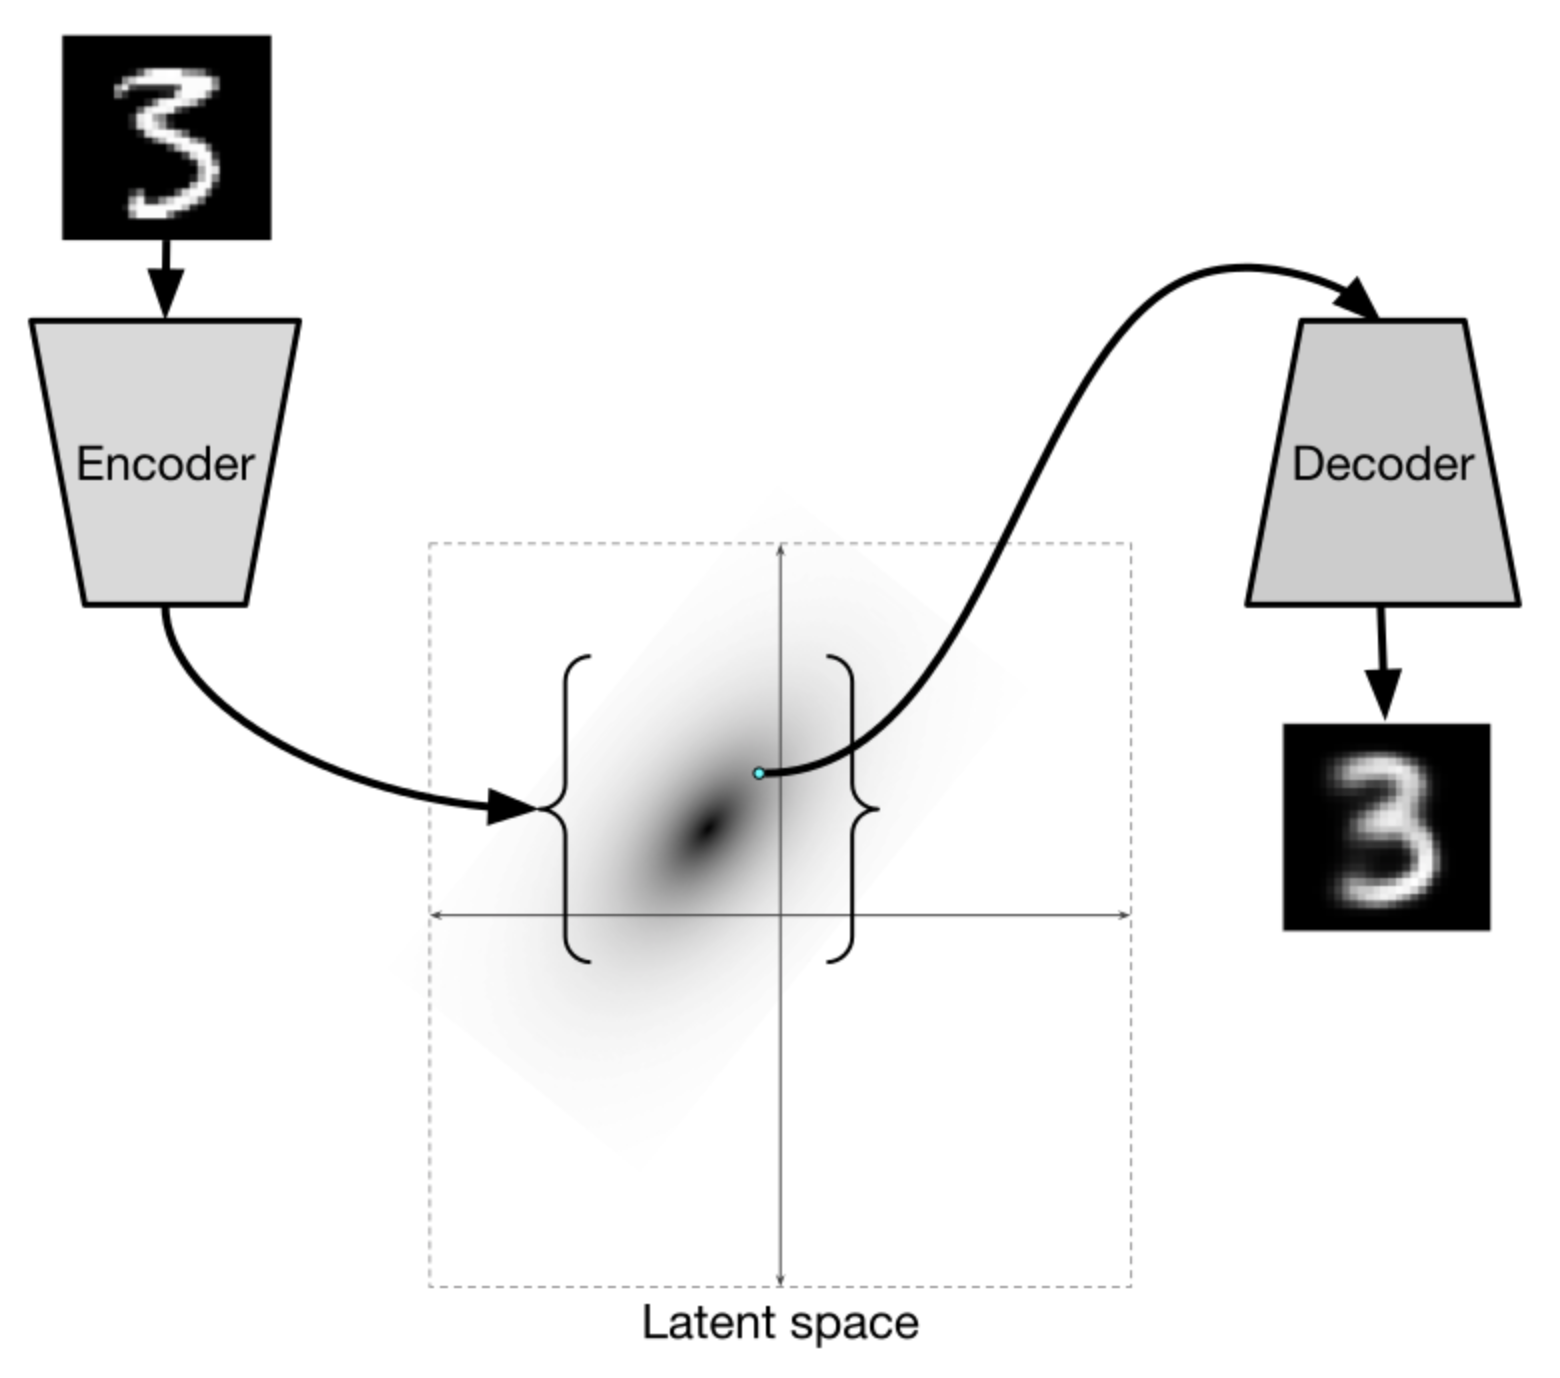
\includegraphics[width=\linewidth]{figs/VAE}
		\end{figure}
	\end{minipage}%
	\begin{minipage}[t]{0.4\columnwidth}
		\begin{figure}[h]
			\centering
			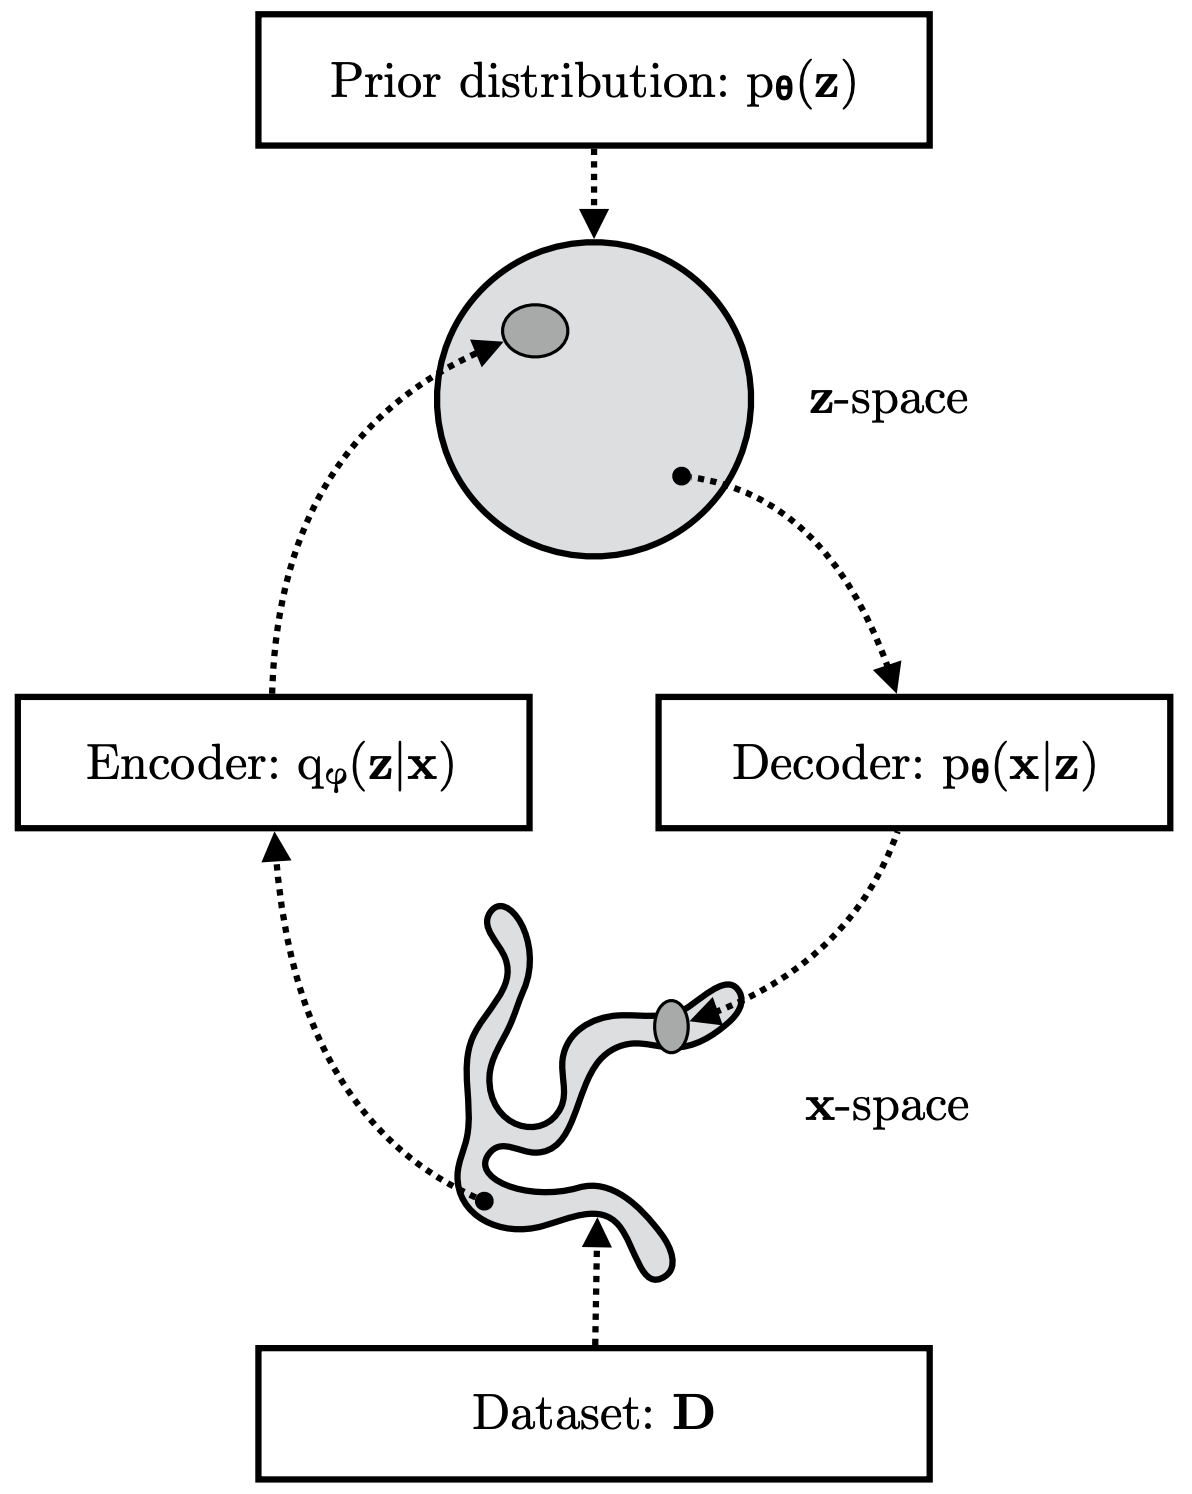
\includegraphics[width=\linewidth]{figs/vae_scheme}
		\end{figure}
	\end{minipage}
\end{frame}
%=======
\begin{frame}{Recap of Previous Lecture}
	\myfootnotewithlink{https://arxiv.org/abs/2007.02731}{Nielsen D., et al. SurVAE Flows: Surjections to Bridge the Gap between VAEs and Flows, 2020}
	\begin{table}[]
		\begin{tabular}{l|c|c}
			& \textbf{VAE} & \textbf{NF} \\ \hline
			\textbf{Objective} & ELBO $\cL$ & Forward KL/MLE \\ \hline
			\textbf{Encoder} & \shortstack{Stochastic \\ $\bz \sim q (\bz | \bx, \bphi)$} &  \shortstack{\\ Deterministic \\ $\bz = \bff_{\btheta}(\bx)$ \\ $q(\bz | \bx, \btheta) = \delta(\bz - \bff_{\btheta}(\bx))$}  \\ \hline
			\textbf{Decoder} & \shortstack{Stochastic \\ $\bx \sim p (\bx | \bz, \btheta)$} & \shortstack{\\ Deterministic \\ $\bx = \bg_{\btheta}(\bz)$ \\ $ p(\bx | \bz, \btheta) = \delta(\bx - \bg_{\btheta}(\bz))$} \\ \hline
			\textbf{Parameters}  & $\bphi, \btheta$ & $\btheta \equiv \bphi$\\ 
		\end{tabular}
	\end{table}
	\begin{block}{Theorem}
		MLE for normalizing flows is equivalent to maximizing the ELBO for a VAE model with deterministic encoder and decoder:
		\vspace{-0.3cm}
		\[
		p(\bx | \bz, \btheta) = \delta (\bx - \bff^{-1}_{\btheta}(\bz)) = \delta (\bx - \bg_{\btheta}(\bz));
		\]
		\[
		q(\bz | \bx, \btheta) = p(\bz | \bx, \btheta) = \delta (\bz - \bff_{\btheta}(\bx)).
		\]
	\end{block}
\end{frame}
%=======
\begin{frame}{Recap of Previous Lecture}
	\myfootnotewithlink{https://arxiv.org/abs/1711.00937}{Oord A., Vinyals O., Kavukcuoglu K. Neural Discrete Representation Learning, 2017} 
	\begin{block}{Assumptions}
		\begin{itemize}
			\item Let $c \sim \Cat(\bpi)$, where 
			\vspace{-0.6cm}
			\[
			\bpi = (\pi_1, \dots, \pi_K), \quad \pi_k = P(c = k), \quad \sum_{k=1}^K \pi_k = 1.
			\]
			\vspace{-0.7cm}
			\item Suppose the VAE includes a discrete latent variable $c$ with prior $p(c) = \text{Uniform}\{1, \dots, K\}$.
		\end{itemize}
	\end{block}
	\begin{block}{ELBO}
		\vspace{-0.6cm}
		\[
			\cL_{\bphi, \btheta}(\bx)  = \bbE_{q(c | \bx, \bphi)} \log p(\bx | c, \btheta) - {\color{olive} \KL(q(c| \bx, \bphi) \| p(c))} \rightarrow \max_{\bphi, \btheta}.
		\]
	\end{block}
	\vspace{-1.0cm}
	\[
		\KL(q(c| \bx, \bphi) \| p(c)) = - \Ent(q(c | \bx, \bphi)) + \log K. 
	\]		
	\vspace{-0.5cm}
	\begin{itemize}
		\item Our encoder must output the discrete distribution $q(c | \bx, \bphi)$.
		\item We'll require an analogue of the reparameterization trick for discrete $q(c | \bx, \bphi)$.
		\item Our decoder $p(\bx | c, \btheta)$ must accept the discrete variable $c$ as input.
	\end{itemize}
\end{frame}
%=======
\begin{frame}{Outline}
	\tableofcontents
\end{frame}
%=======
\section{Vector Quantization: Discrete VAE Latent Representations}
%=======
\begin{frame}{Vector Quantization}
	\myfootnotewithlink{https://arxiv.org/abs/2004.02088}{Zhao Y. et al. Feature Quantization Improves GAN Training, 2020} 
	Define the codebook (dictionary) space $\{\be_k\}_{k=1}^K$ with $\be_k \in \bbR^L$ and $K$ the number of codebook entries.
	\begin{block}{Quantized Representation}
		A quantized vector $\bz_q \in \bbR^{L}$, for any $\bz \in \bbR^L$, is defined via nearest-neighbor lookup in the codebook:
		\vspace{-0.3cm}
		\[
		\bz_q = \bq (\bz) = \be_{k^*}, \quad \text{where } k^* = \argmin_k \| \bz - \be_k \|.
		\] 
		\vspace{-0.7cm}
	\end{block}
	\vspace{-0.2cm}
	\begin{block}{Quantization Procedure}
		If the encoded tensor has spatial dimensions, quantization is independently applied to each of the $W \times H$ locations.
		\begin{minipage}[t]{0.65\columnwidth}
			\begin{figure}
				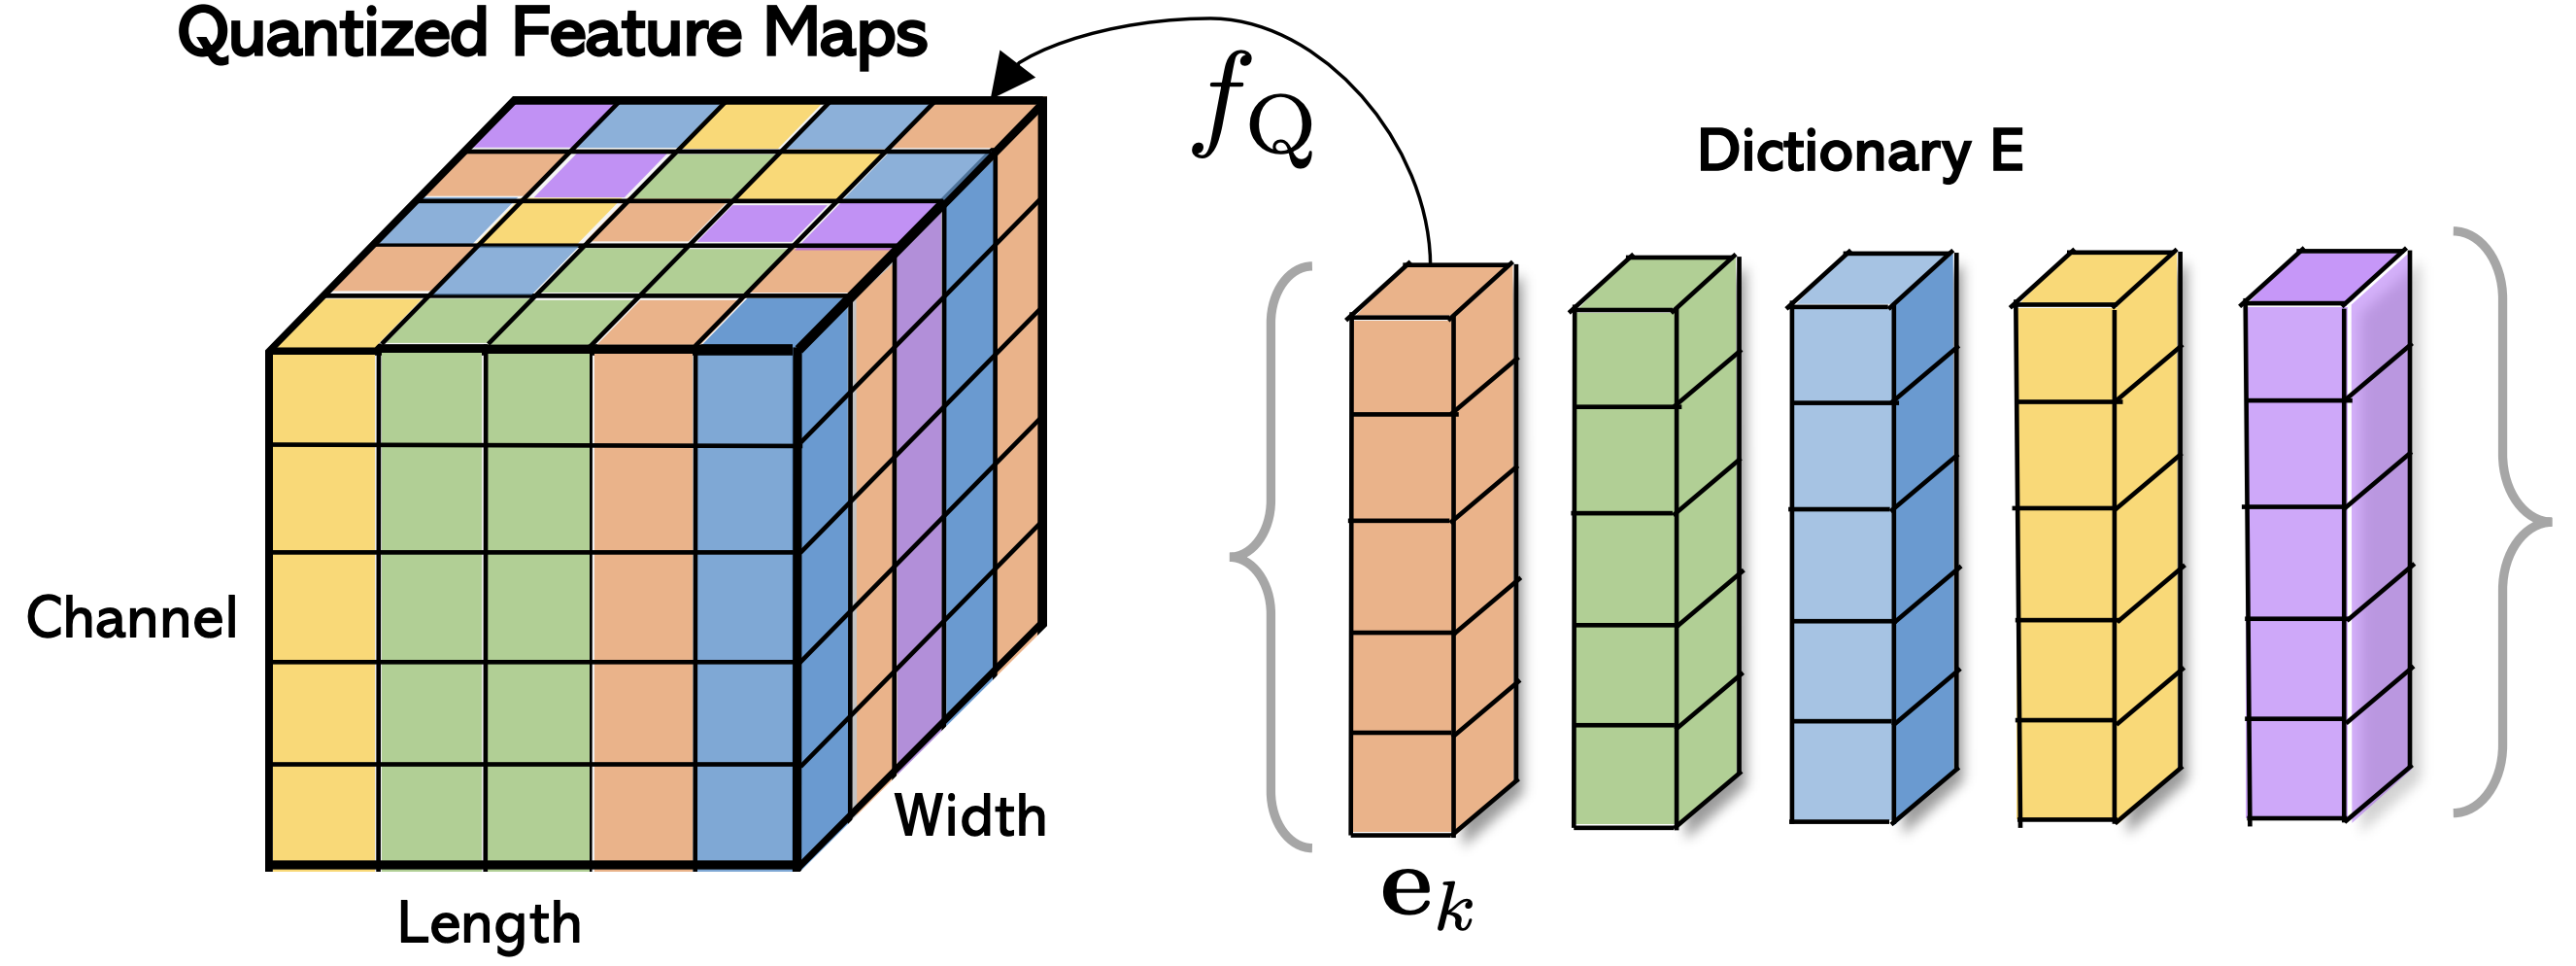
\includegraphics[width=0.8\linewidth]{figs/fqgan_cnn.png}
			\end{figure}
		\end{minipage}%
		\begin{minipage}[t]{0.35\columnwidth}
			\begin{figure}
				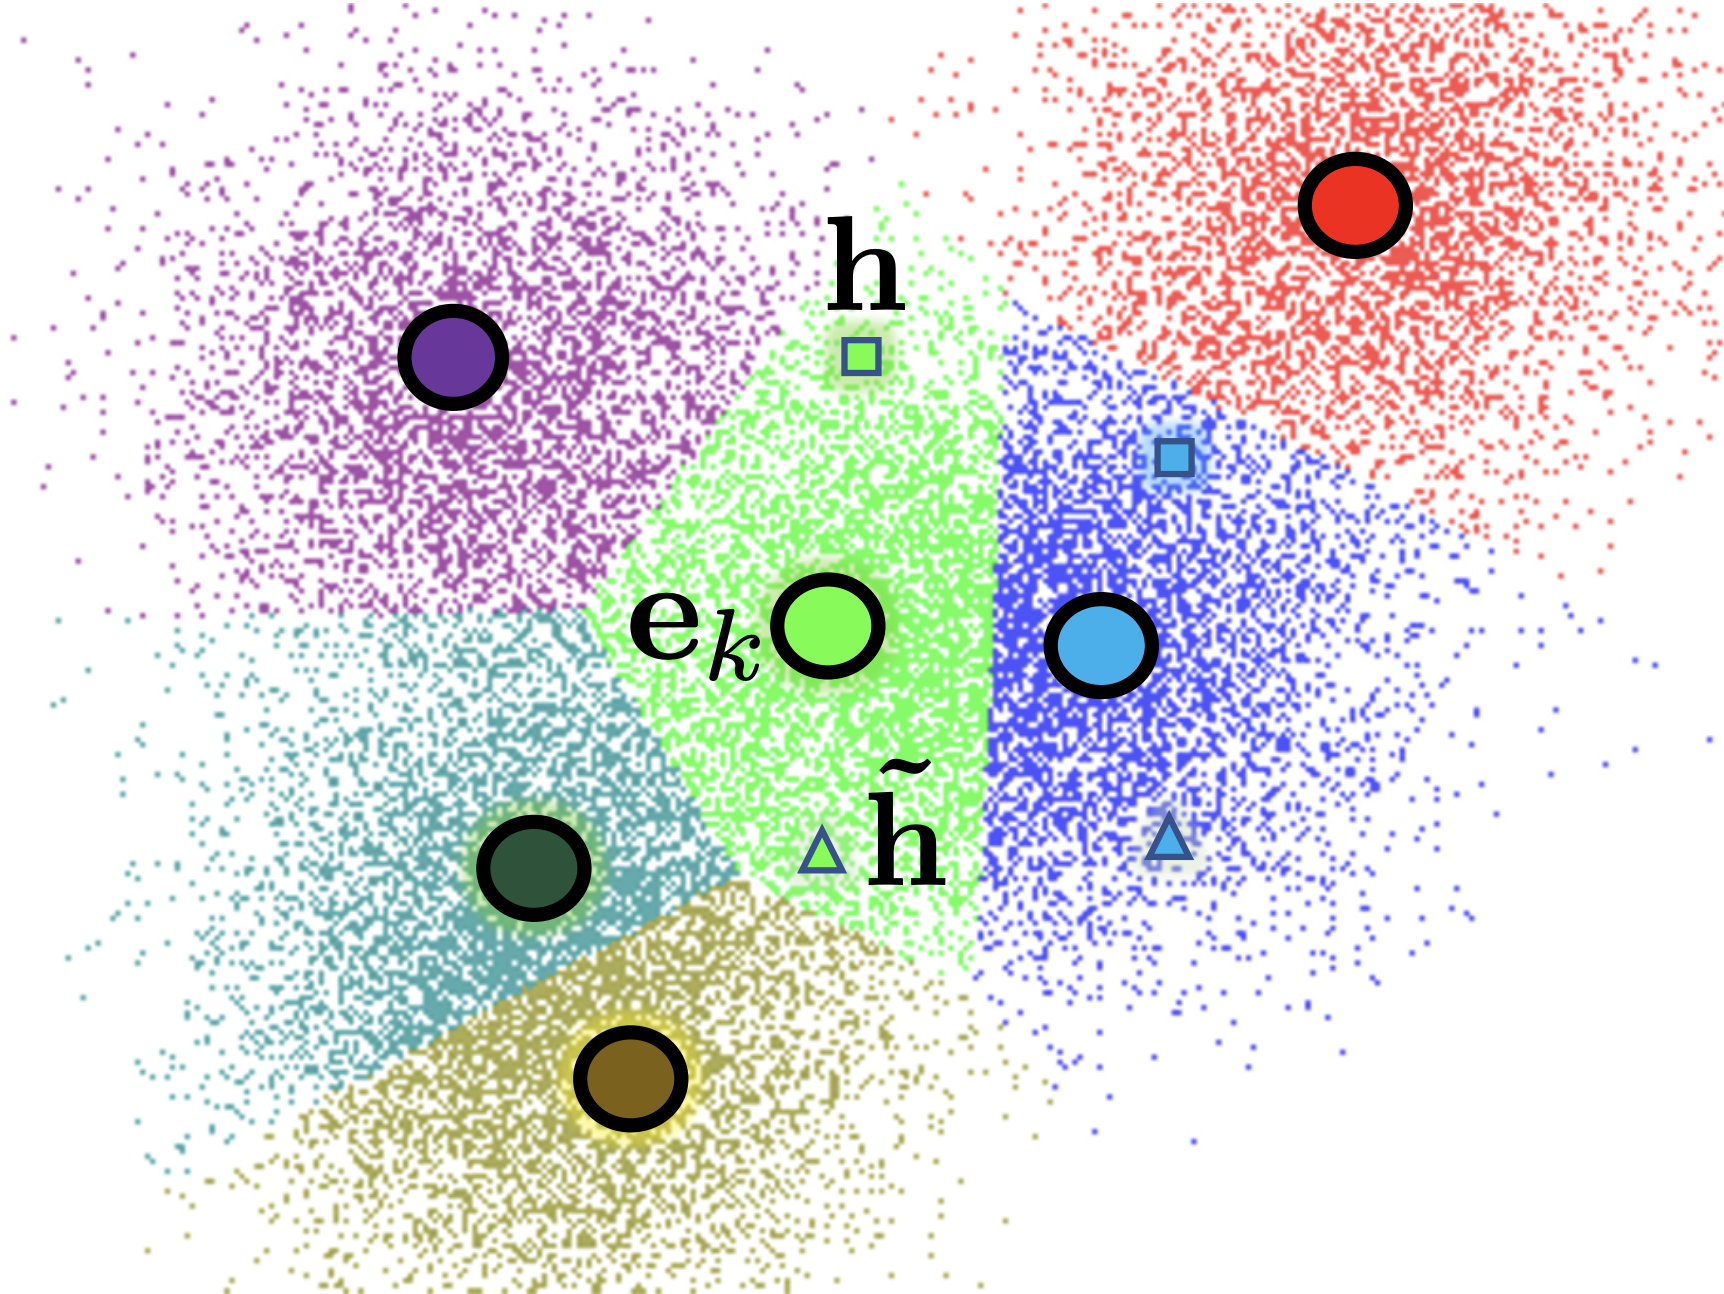
\includegraphics[width=0.7\linewidth]{figs/fqgan_lookup}
			\end{figure}
		\end{minipage}
	\end{block}
\end{frame}
%=======
\begin{frame}{Vector Quantized VAE (VQ-VAE)}
	\myfootnotewithlink{https://arxiv.org/abs/1711.00937}{Oord A., Vinyals O., Kavukcuoglu K. Neural Discrete Representation Learning, 2017} 
	\begin{itemize}
		\item The encoder outputs a continuous vector $\bz_e = \text{NN}_{e, \bphi}(\bx) \in \bbR^{L}$.
		\item Quantization deterministically maps $\bz_e$ to its quantized codebook vector $\bz_q$.
		\item The decoder is conditioned on codebook entries $\be_c$, i.e., via $p(\bx | \be_c, \btheta)$ (instead of $p(\bx | c, \btheta)$).
	\end{itemize}
	\begin{block}{Deterministic Variational Posterior}
		\vspace{-0.3cm}
		\[
			q(c = k^* | \bx, \bphi) = \begin{cases}
				1 , \quad \text{for } k^* = \argmin_k \| \bz_e - \be_k \|; \\
				0, \quad \text{otherwise}.
		\end{cases}
		\]
		\[
			\KL(q(c | \bx, \bphi) \| p(c)) = - \underbrace{\Ent(q(c | \bx, \bphi))}_{=0} + \log K = \log K. 
		\]
	\end{block}	
	\vspace{-0.4cm}
	\textbf{Note:} The KL regularizer becomes constant and has no direct effect on the ELBO objective in this case.
\end{frame}
%=======
\begin{frame}{Vector Quantized VAE (VQ-VAE): Forward}
	\myfootnotewithlink{https://arxiv.org/abs/1711.00937}{Oord A., Vinyals O., Kavukcuoglu K. Neural Discrete Representation Learning, 2017} 
	\begin{block}{Deterministic Variational Posterior}
		\vspace{-0.3cm}
		\[
			q(c = k^* | \bx, \bphi) = \begin{cases}
			1 , \quad \text{if } k^* = \argmin_k \| \bz_e - \be_k \|; \\
			0, \quad \text{otherwise}.
			\end{cases}
		\]
	\vspace{-0.5cm}
	\end{block}	
	\begin{block}{ELBO}
		\vspace{-0.6cm}
		\[
		\cL_{\bphi, \btheta}(\bx)  = \bbE_{q(c | \bx, \bphi)} \log p(\bx | \be_{c} , \btheta) - \log K =  \log p(\bx | \bz_q, \btheta) - \log K,
		\]
		where $\bz_q = \be_{k^*}$, $k^* = \argmin_k \| \bz_e - \be_k \|$.
	\end{block}
	\vspace{-0.3cm} 
	\begin{figure}
		\centering
		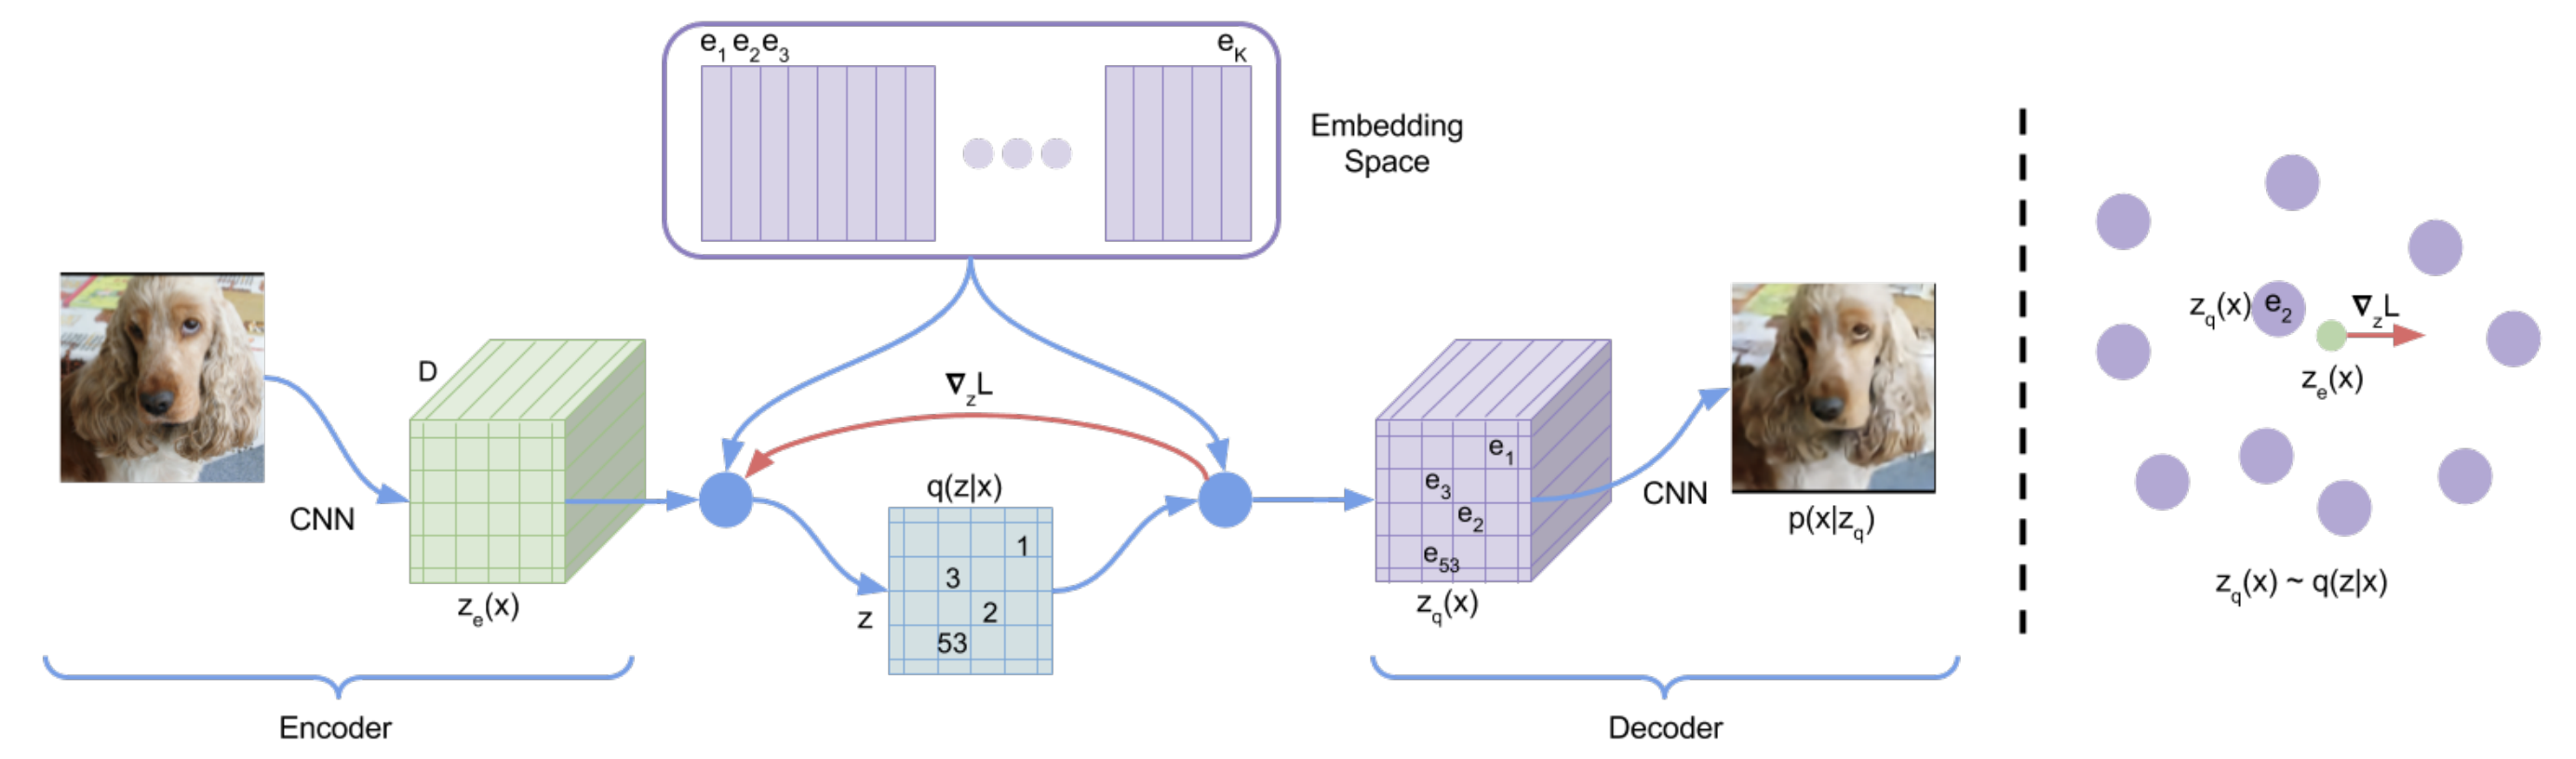
\includegraphics[width=0.85\linewidth]{figs/vqvae}
	\end{figure}
	\vspace{-0.3cm} 
	\textbf{Challenge:} The $\argmin$ operation is non-differentiable.
\end{frame}
%=======
\begin{frame}{Vector Quantized VAE (VQ-VAE): Backward}
	\myfootnotewithlink{https://arxiv.org/abs/1711.00937}{Oord A., Vinyals O., Kavukcuoglu K. Neural Discrete Representation Learning, 2017} 
	\begin{block}{ELBO}
		\vspace{-0.5cm}
		\[
			\cL_{\bphi, \btheta}(\bx)  =  \log p(\bx | \bz_q, \btheta) - \log K, \quad \bz_q = \be_{k^*},\; k^* = \argmin_k \| \bz_e - \be_k \|.
		\]
		\vspace{-0.5cm}
	\end{block}
	\begin{figure}
		\centering
		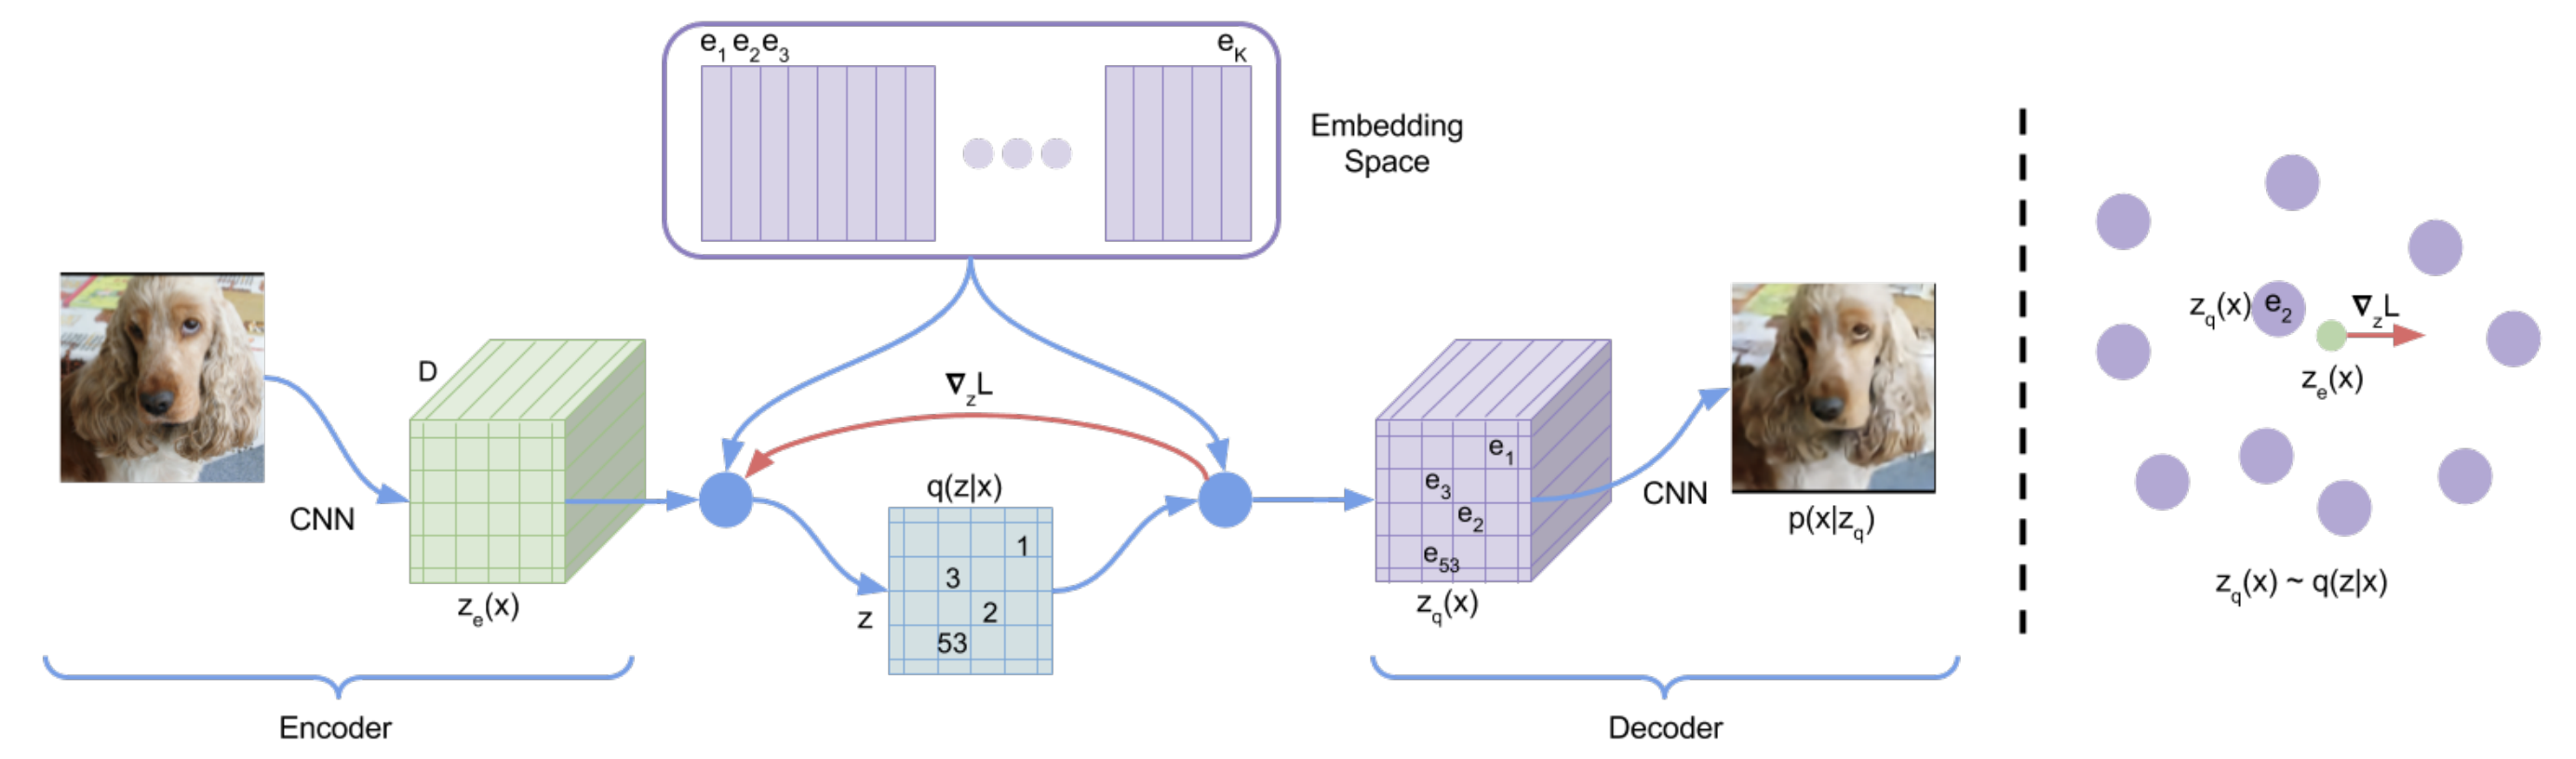
\includegraphics[width=0.85\linewidth]{figs/vqvae}
	\end{figure}
	\vspace{-0.3cm}
	\begin{block}{Straight-Through Gradient Estimator}
		\vspace{-0.5cm}
		\begin{multline*}
		\frac{\partial \log p(\bx | \bz_q , \btheta)}{\partial \bphi} = \frac{\partial \log p(\bx | \bz_q, \btheta)}{\partial \bz_q} \cdot {\color{red}\frac{\partial \bz_q}{\partial \bphi}} = \\
		= \frac{\partial \log p(\bx | \bz_q, \btheta)}{\partial \bz_q} \cdot {\color{red}\frac{\partial \bz_q}{\partial \bz_e}} \cdot \frac{\partial \bz_e}{\partial \bphi} \approx \frac{\partial \log p(\bx | \bz_q, \btheta)}{\partial \bz_q} \cdot \frac{\partial \bz_e}{\partial \bphi}
		\end{multline*}
	\end{block}
\end{frame}
%=======
\begin{frame}{Vector Quantized VAE-2 (VQ-VAE-2)}
	\myfootnotewithlink{https://arxiv.org/abs/1906.00446}{Razavi A., Oord A., Vinyals O. Generating Diverse High-Fidelity Images with VQ-VAE-2, 2019} 
	Extension to the spatial domain: $\bc \in \{1, \dots, K\}^{W \times H}$
	\vspace{-0.3cm}
	\[
		q(\bc | \bx, \bphi) = \prod_{i=1}^W \prod_{j=1}^H q(c_{ij} | \bx, \bphi); \quad p(\bc) = \prod_{i=1}^W \prod_{j=1}^H \text{Uniform}\{1, \dots, K\}.
	\]
	\vspace{-0.6cm}
	\begin{block}{Sample Diversity}
		\vspace{-0.2cm}
		\begin{figure}
			\centering
			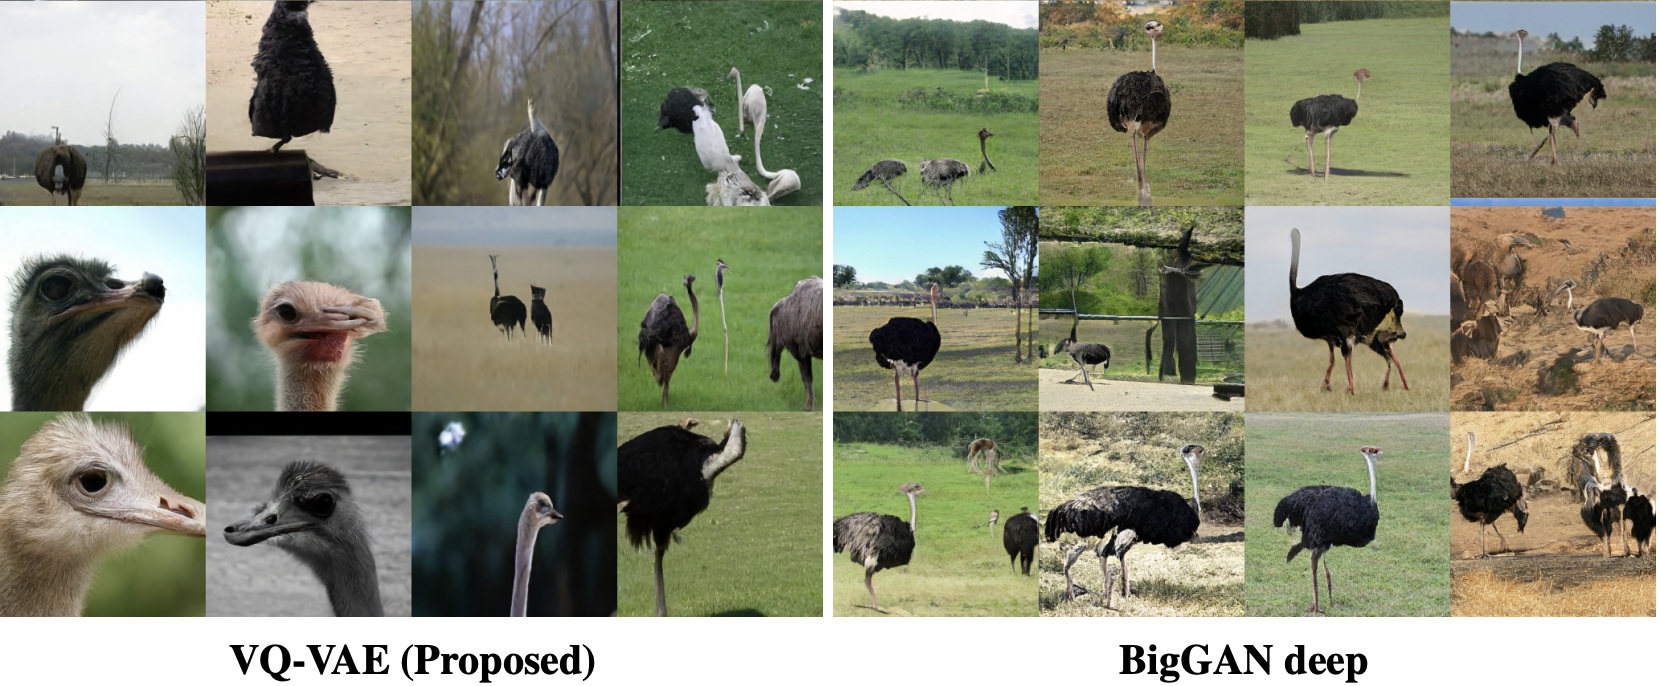
\includegraphics[width=1.0\linewidth]{figs/vqvae2_diversity}
		\end{figure}
	\end{block}
\end{frame}
%=======
\section{ELBO Surgery}
%=======
\begin{frame}{ELBO Surgery}
	\myfootnotewithlink{http://approximateinference.org/accepted/HoffmanJohnson2016.pdf}{Hoffman M. D., Johnson M. J. ELBO Surgery: Yet Another Way to Carve Up the Variational Evidence Lower Bound, 2016}
	\vspace{-0.3cm}
	\[
	    \frac{1}{n} \sum_{i=1}^n \cL_{\bphi, \btheta}(\bx_i) = \frac{1}{n} \sum_{i=1}^n \Bigl[ \bbE_{q(\bz | \bx_i, \bphi)} \log p(\bx_i | \bz, \btheta) - \KL(q(\bz | \bx_i, \bphi) \| p(\bz)) \Bigr].
	\]
	\vspace{-0.3cm}
	\begin{block}{Theorem}
		\vspace{-0.5cm}
		\[
		    \frac{1}{n} \sum_{i=1}^n \KL(q(\bz | \bx_i, \bphi) \| p(\bz)) = {\color{violet} \KL(q_{\text{agg}}(\bz | \bphi) \| p(\bz))} + {\color{teal}\bbI_{q} [\bx, \bz]};
		\]
		\vspace{-0.5cm}
		\begin{itemize}
			\item $q_{\text{agg}}(\bz | \bphi) = \frac{1}{n} \sum_{i=1}^n q(\bz | \bx_i, \bphi)$ denotes the \textbf{aggregated} variational posterior.
			\item $\bbI_{q} [\bx, \bz]$ is the mutual information between $\bx$ and $\bz$ under the data distribution $\pi(\bx)$ and $q(\bz | \bx, \bphi)$.
			\item  {\color{violet} The first term} encourages $q_{\text{agg}}(\bz | \bphi)$ to match the prior $p(\bz)$.
			\item {\color{teal} The second term} reduces the information about $\bx$ encoded in~$\bz$.
		\end{itemize}
	\end{block}
\end{frame}
%=======
\begin{frame}{ELBO Surgery}
	\myfootnotewithlink{http://approximateinference.org/accepted/HoffmanJohnson2016.pdf}{Hoffman M. D., Johnson M. J. ELBO Surgery: Yet Another Way to Carve Up the Variational Evidence Lower Bound, 2016}
		\vspace{-0.4cm}
		\[
		    \frac{1}{n} \sum_{i=1}^n \KL(q(\bz | \bx_i, \bphi) \| p(\bz)) = \KL(q_{\text{agg}}(\bz | \bphi) \| p(\bz)) + \bbI_q [\bx, \bz].
		\]
		\vspace{-0.3cm}
	\begin{block}{Proof}
		\vspace{-0.5cm}
		{\footnotesize
		\begin{multline*}
		    \frac{1}{n} \sum_{i=1}^n \KL(q(\bz | \bx_i, \bphi) \| p(\bz)) = \frac{1}{n} \sum_{i=1}^n \int q(\bz | \bx_i, \bphi) \log \frac{q(\bz | \bx_i, \bphi)}{p(\bz)} d \bz = \\
		    = \frac{1}{n} \sum_{i=1}^n \int q(\bz | \bx_i, \bphi) \log \frac{{\color{violet}q_{\text{agg}}(\bz | \bphi)} {\color{teal}q(\bz | \bx_i, \bphi)}}{{\color{violet}p(\bz)} {\color{teal}q_{\text{agg}}(\bz | \bphi)}} d \bz = \\
		    = \int \frac{1}{n} \sum_{i=1}^n  q(\bz | \bx_i, \bphi) \log {\color{violet}\frac{q_{\text{agg}}(\bz | \bphi)}{p(\bz)}} d \bz
		    + \frac{1}{n}\sum_{i=1}^n \int q(\bz | \bx_i, \bphi) \log {\color{teal}\frac{q(\bz | \bx_i, \bphi)}{q_{\text{agg}}(\bz | \bphi)}} d \bz = \\
		    = \KL (q_{\text{agg}}(\bz | \bphi) \| p(\bz)) + \frac{1}{n}\sum_{i=1}^n \KL(q(\bz | \bx_i, \bphi) \| q_{\text{agg}}(\bz | \bphi))
		\end{multline*}
		}
		\vspace{-0.4cm}
		\[
			\bbI_{q} [\bx, \bz] = \frac{1}{n}\sum_{i=1}^n \KL(q(\bz | \bx_i, \bphi) \| q_{\text{agg}}(\bz | \bphi)).
		\]
	\end{block}
\end{frame}
%=======
\begin{frame}{ELBO Surgery}
	\myfootnotewithlink{http://approximateinference.org/accepted/HoffmanJohnson2016.pdf}{Hoffman M. D., Johnson M. J. ELBO Surgery: Yet Another Way to Carve Up the Variational Evidence Lower Bound, 2016}
	\vspace{-0.3cm}
	\begin{block}{Revisiting the ELBO}
		\vspace{-0.7cm}
		{\small
		\begin{multline*}
		    \frac{1}{n}\sum_{i=1}^n \cL_{\bphi, \btheta}(\bx_i) = \frac{1}{n} \sum_{i=1}^n \left[ \bbE_{q(\bz | \bx_i, \bphi)} \log p(\bx_i | \bz, \btheta) - \KL(q(\bz | \bx_i, \bphi) \| p(\bz)) \right] = \\
		    = \underbrace{\frac{1}{n} \sum_{i=1}^n \bbE_{q(\bz | \bx_i, \bphi)} \log p(\bx_i | \bz, \btheta)}_{\text{Reconstruction Loss}} - \underbrace{\vphantom{ \sum_{i=1}^n} \bbI_q [\bx, \bz]}_{\text{Mutual Information}} - \underbrace{\vphantom{ \sum_{i=1}^n} \KL(q_{\text{agg}}(\bz | \bphi) \| {\color{teal}p(\bz)})}_{\text{Marginal KL}}
		\end{multline*}
		}
		\vspace{-0.3cm}
	\end{block}
	The prior distribution $p(\bz)$ only appears in the last term.
	\begin{block}{Optimal VAE Prior}
		\vspace{-0.7cm}
		\[
	  		\KL(q_{\text{agg}}(\bz | \bphi) \| p(\bz)) = 0 \quad \Leftrightarrow \quad p (\bz) = q_{\text{agg}}(\bz | \bphi) = \frac{1}{n} \sum_{i=1}^n q(\bz | \bx_i, \bphi).
		\]
		\vspace{-0.4cm} \\
		Hence, the optimal prior $p(\bz)$ is the aggregated variational posterior $q_{\text{agg}}(\bz | \bphi)$.
	\end{block}
	
\end{frame}
%=======
\begin{frame}{Marginal KL}
	\myfootnotewithlink{https://arxiv.org/abs/1505.05770}{Rezende D. J., Mohamed S. Variational Inference with Normalizing Flows, 2015} 
	\[
		\KL(q_{\text{agg}}(\bz | \bphi) \| p(\bz))
	\]
	\vspace{-0.5cm}
	\begin{itemize}
		\item $q(\bz | \bx, \bphi) = \cN(\bmu_{\bphi}(\bx), \bsigma^2_{\bphi}(\bx))$ is unimodal. 
		\item It is generally believed that the \textbf{mismatch between} $p(\bz)$  \textbf{and} $q_{\text{agg}}(\bz | \bphi)$  is the primary explanation for blurry VAE-generated images.
	\end{itemize}
	\begin{figure}
		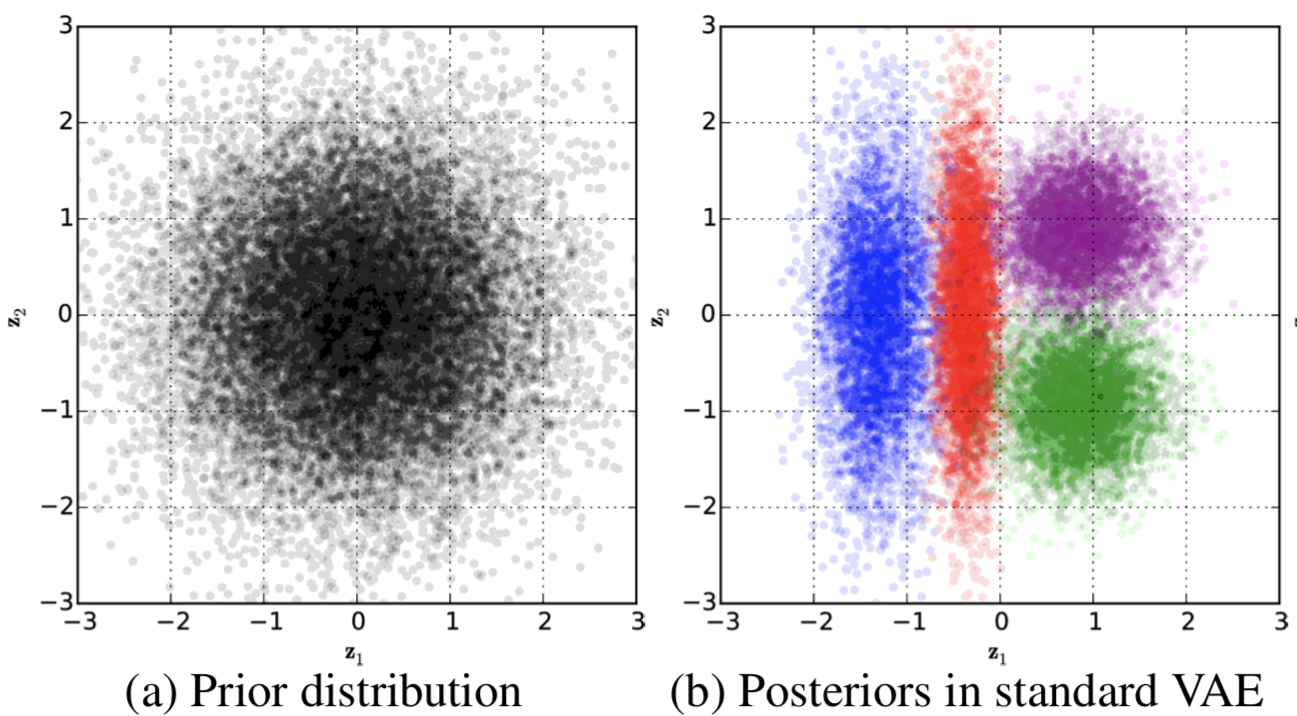
\includegraphics[width=0.8\linewidth]{figs/agg_posterior}
	\end{figure}
\end{frame}
%=======
\section{Learnable VAE Prior}
%=======
\begin{frame}{Optimal VAE Prior}
	\myfootnotewithlink{https://jmtomczak.github.io/blog/7/7\_priors.html}{image credit: https://jmtomczak.github.io/blog/7/7\_priors.html}
	\begin{itemize}
		\item Standard Gaussian $p(\bz) = \cN(0, \bI)$ often leads to over-regularization.
		\item $p(\bz) = q_{\text{agg}}(\bz | \bphi) = \frac{1}{n}\sum_{i=1}^n q(\bz | \bx_i, \bphi)$ risks overfitting and incurs high computational cost.
	\end{itemize}
	\vspace{-0.5cm}
	\begin{minipage}[t]{0.5\columnwidth}
		\begin{block}{Non-Learnable Prior $p(\bz)$}
			\begin{figure}[h]
				\centering
				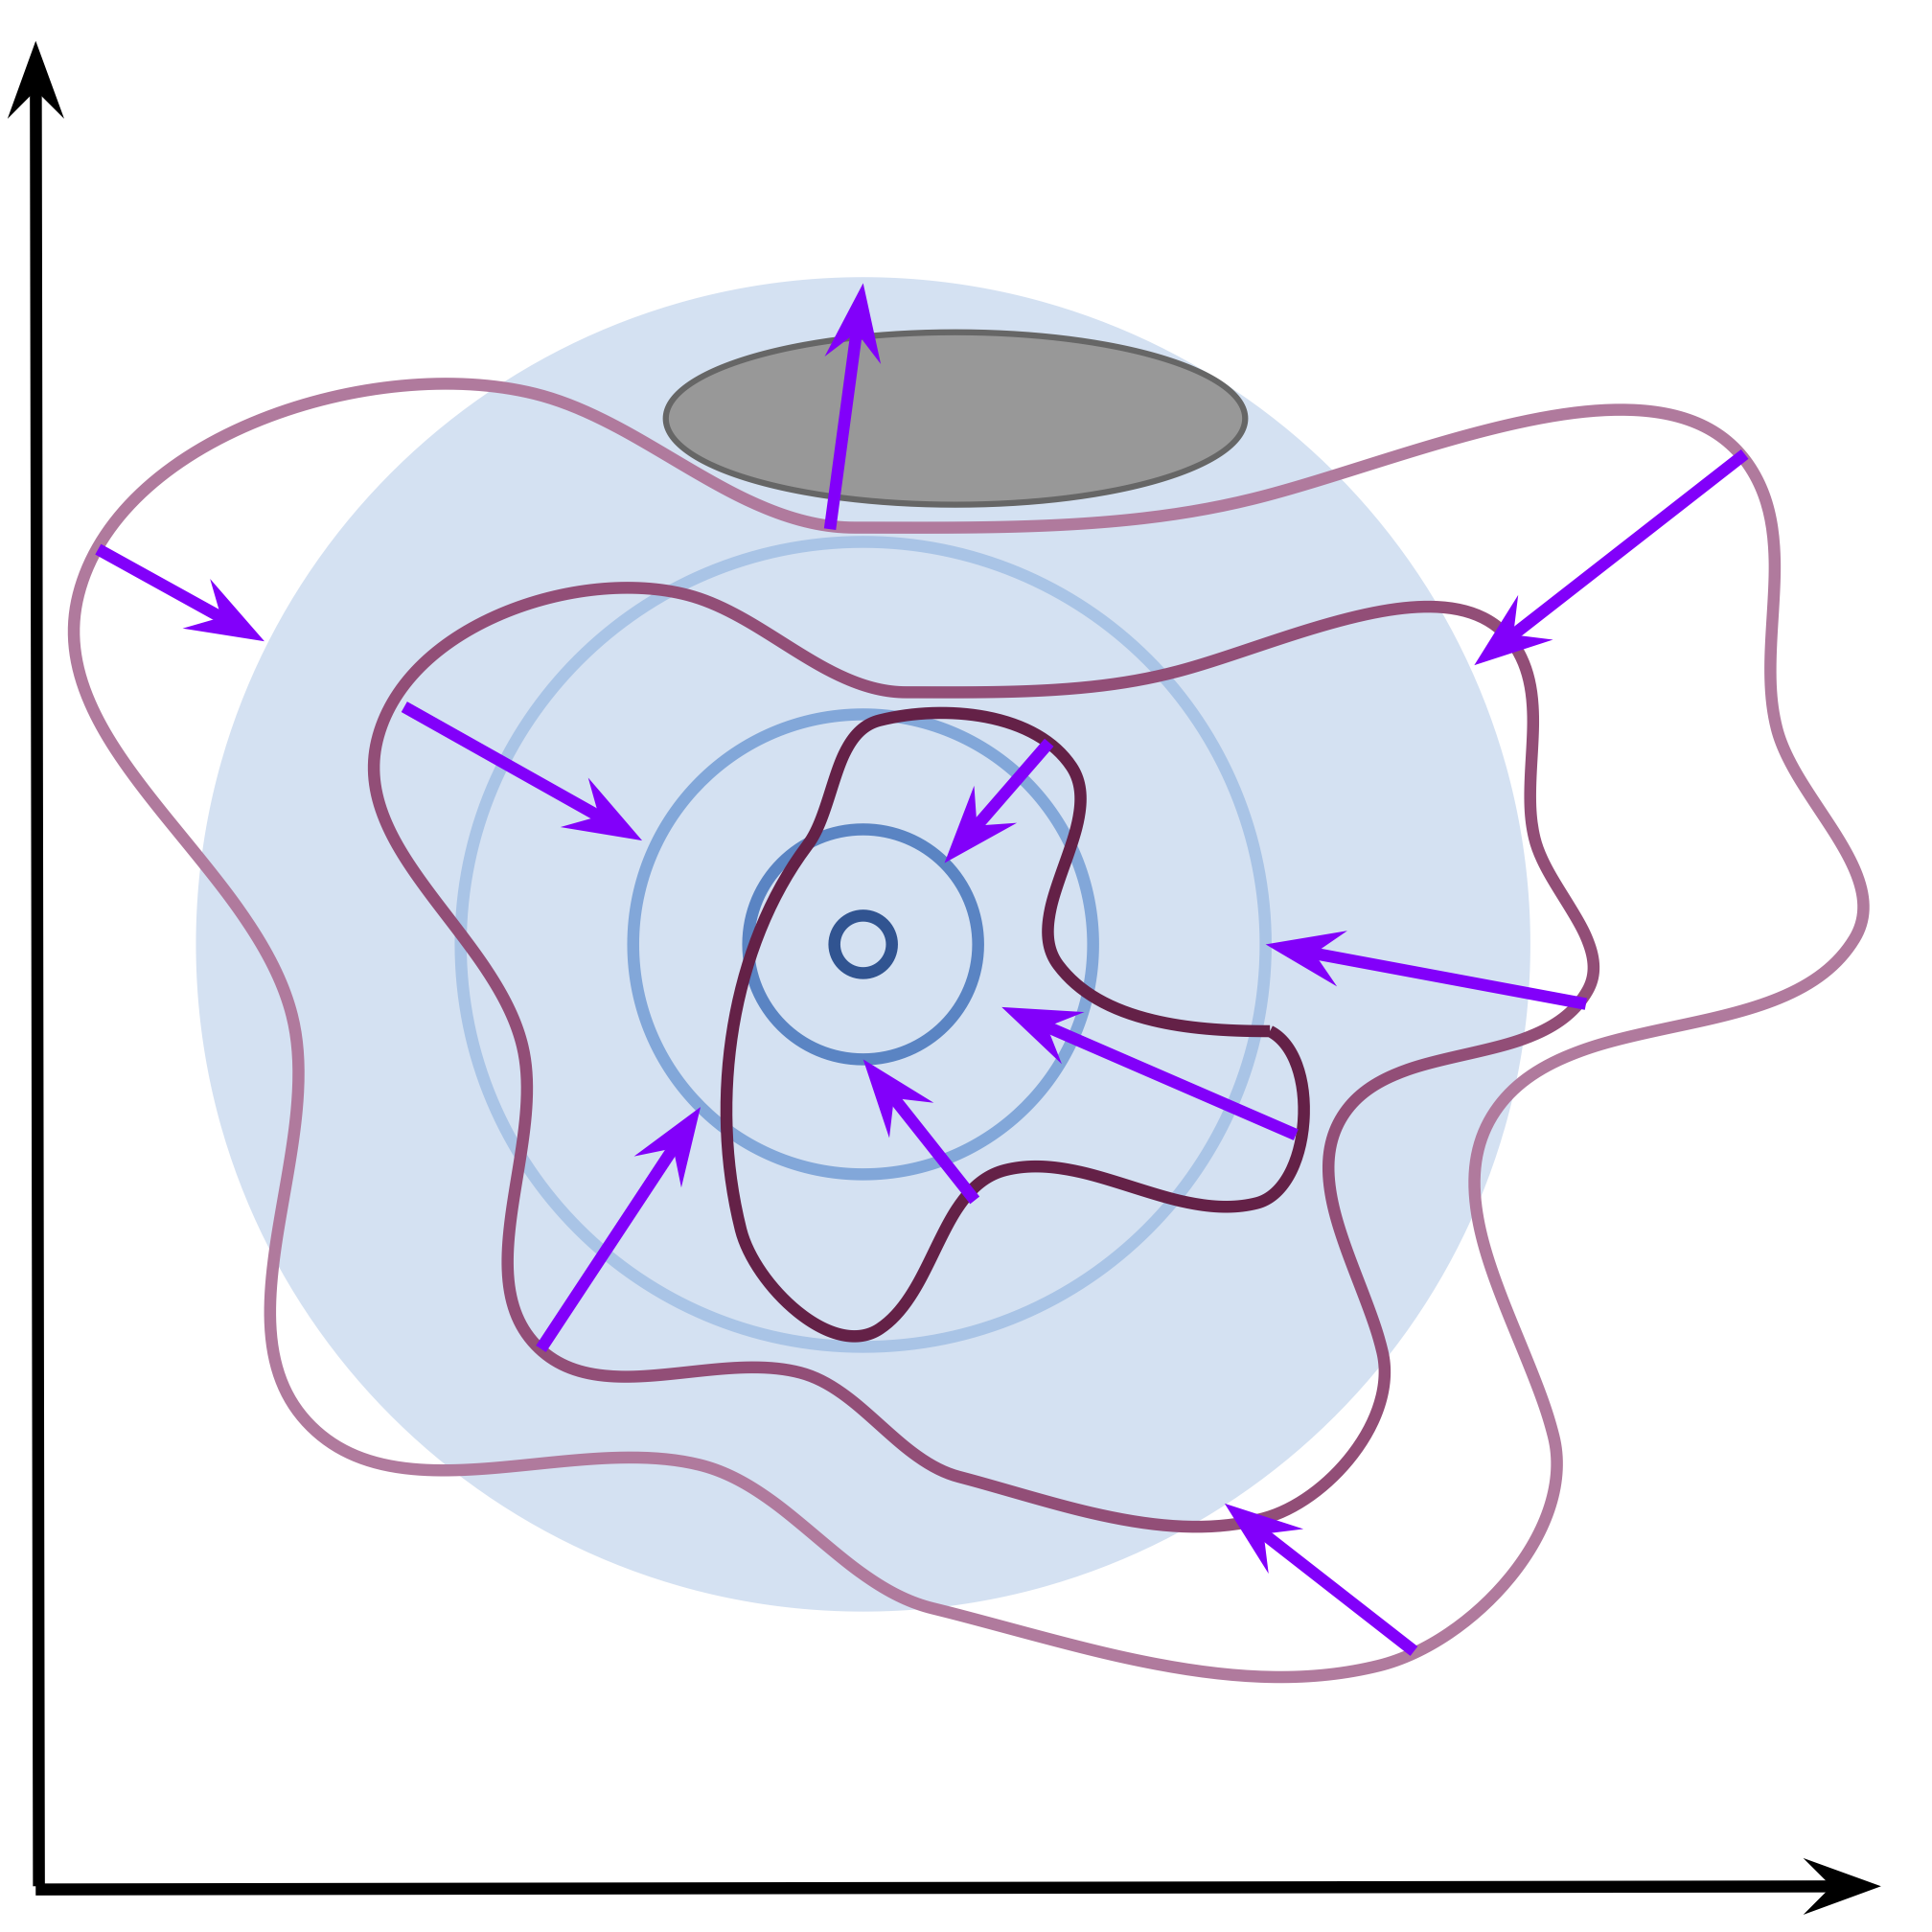
\includegraphics[width=0.6\linewidth]{figs/non_learnable_prior}
			\end{figure}
		\end{block}
	\end{minipage}%
	\begin{minipage}[t]{0.5\columnwidth}
		\begin{block}{Learnable Prior $p(\bz | \blambda)$}
			\begin{figure}[h]
				\centering
				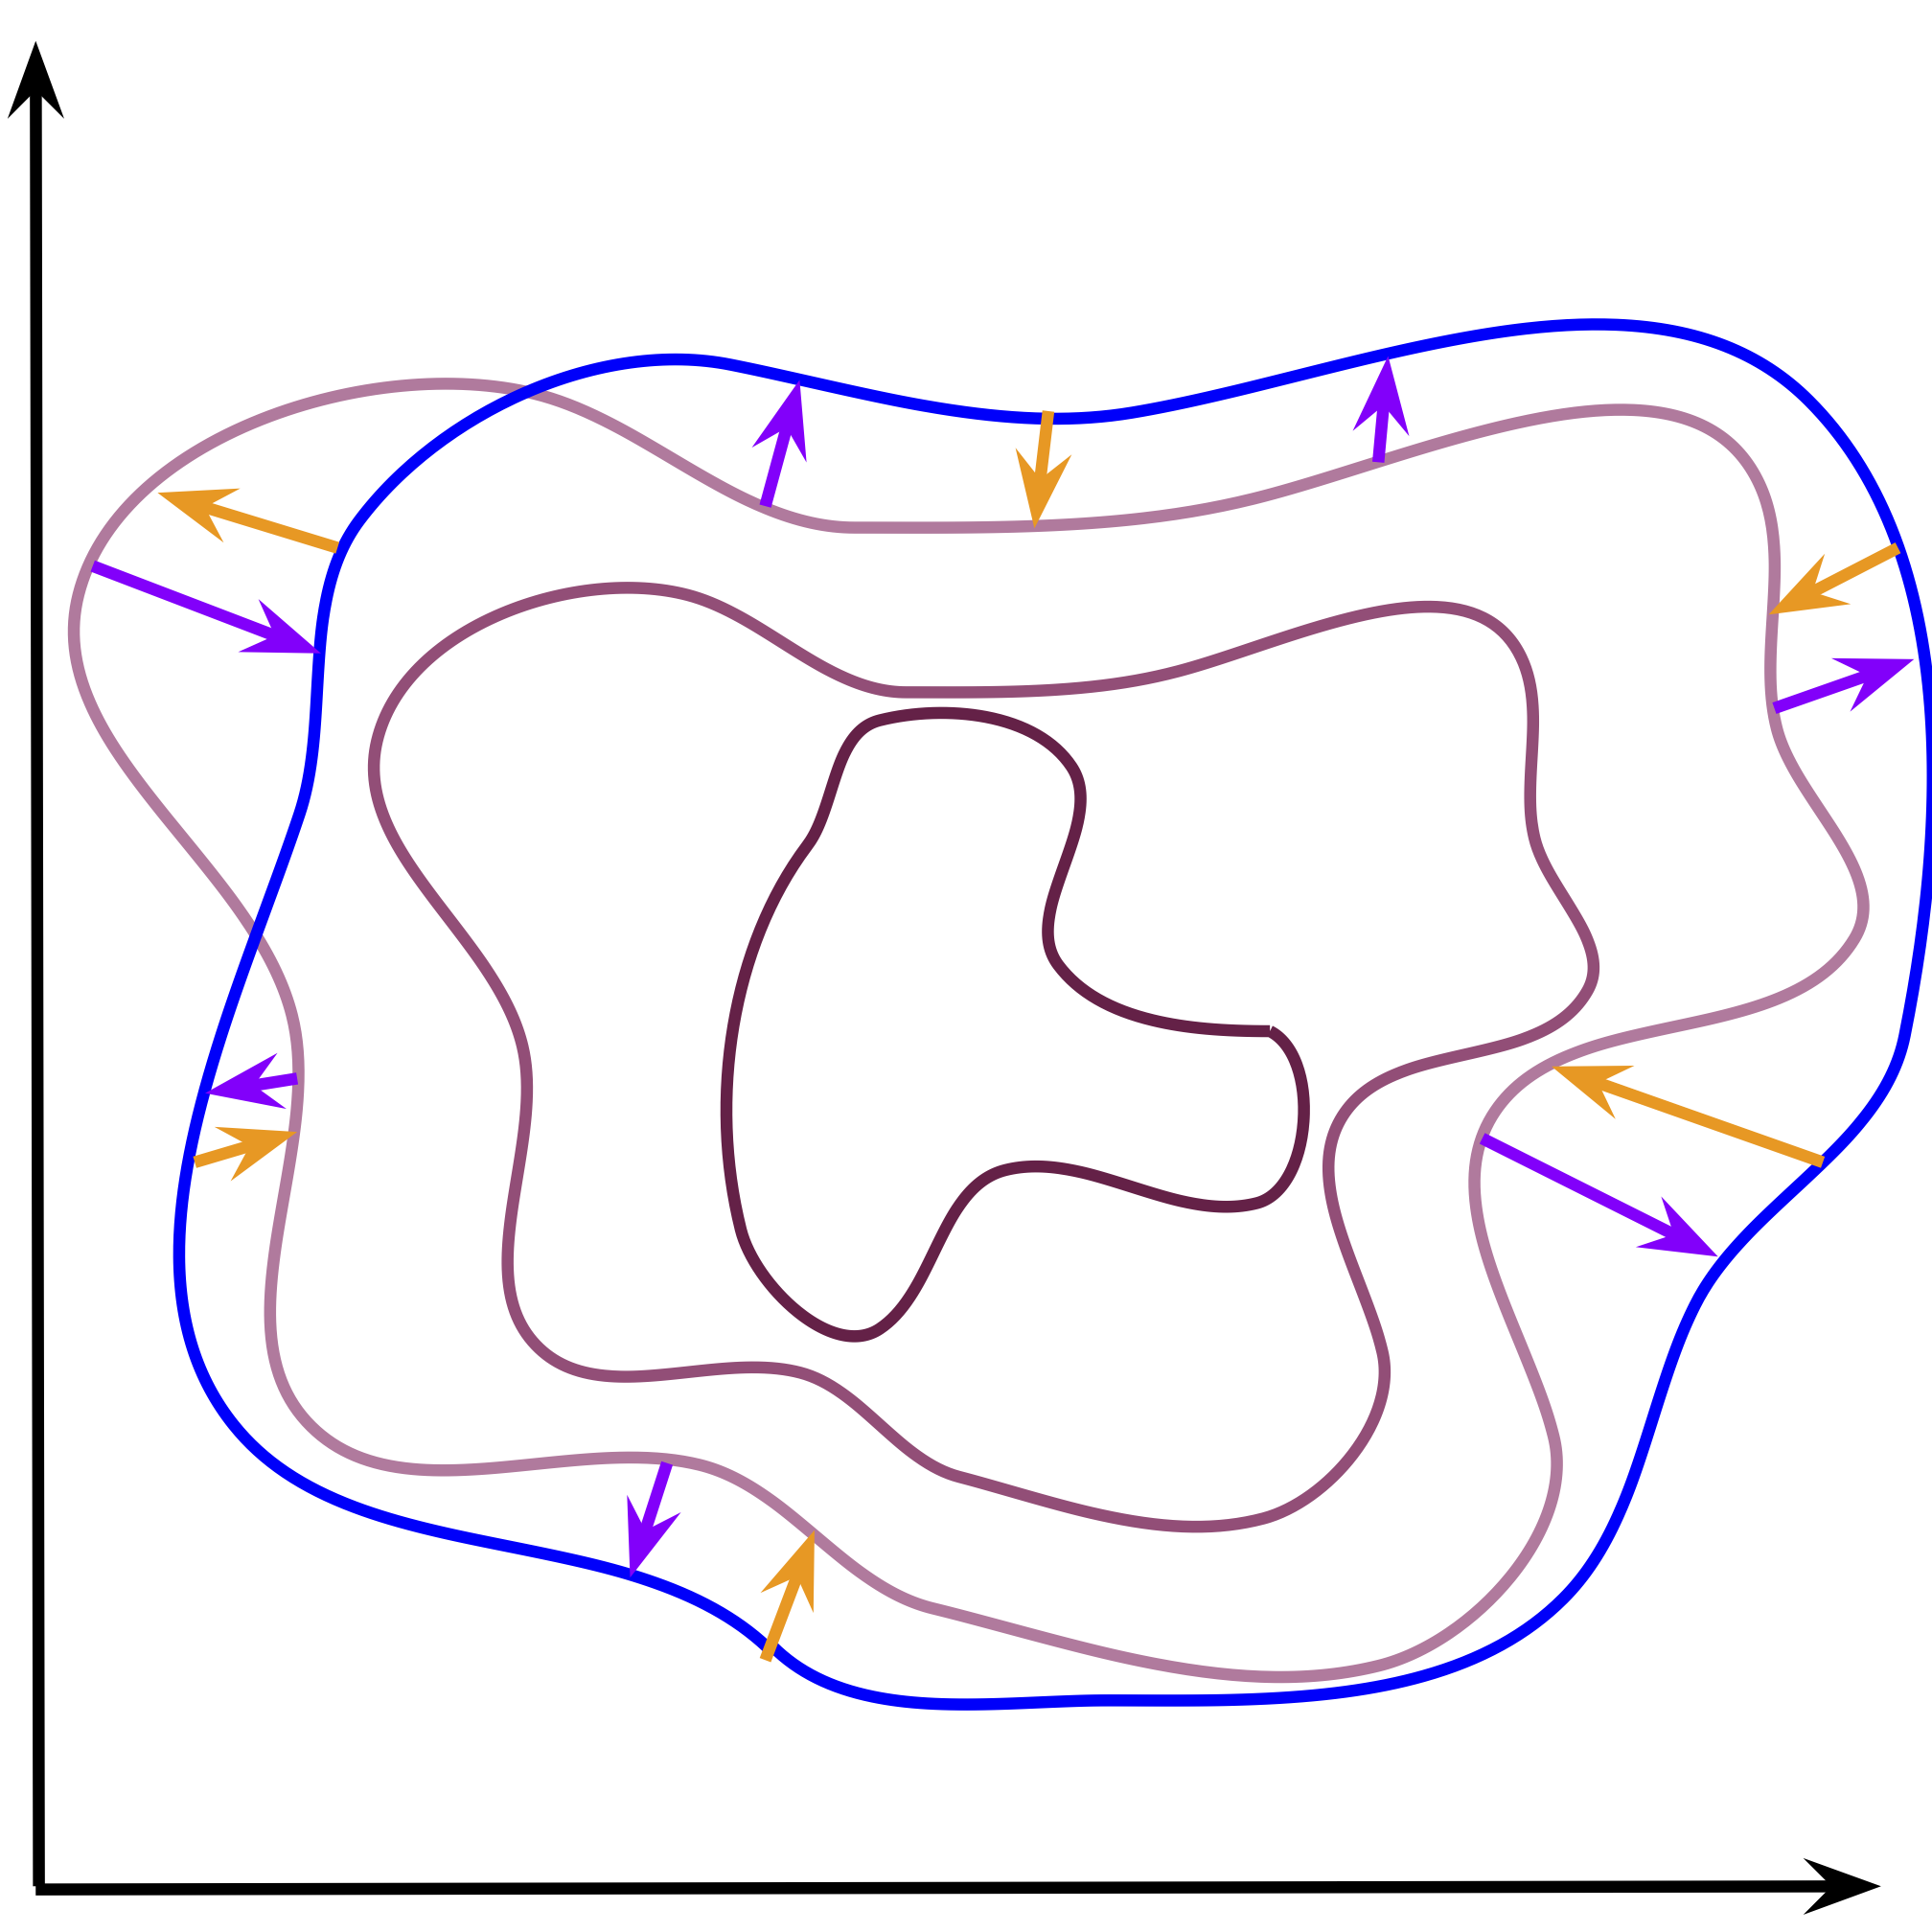
\includegraphics[width=0.6\linewidth]{figs/learnable_prior}
			\end{figure}
		\end{block}
	\end{minipage}
	\vspace{-0.3cm}
	\[
	\frac{1}{n}\sum_{i=1}^n \cL_{\bphi, \btheta}(\bx_i) = \text{RL} - \text{MI} -  \KL(q_{\text{agg}}(\bz | \bphi) \| {\color{teal}p(\bz | \blambda)})
	\]
	This is the forward KL divergence with respect to $p(\bz | \blambda)$.
\end{frame}
%=======
\begin{frame}{NF-Based VAE Prior}
	\myfootnotewithlink{https://arxiv.org/abs/1611.02731}{Chen X. et al. Variational Lossy Autoencoder, 2016}
	\begin{block}{NF Model in Latent Space}
		\vspace{-0.5cm}
		\[
		\log p(\bz | \blambda) = \log p(\bz^*) + \log  \left | \det \left(\frac{d \bz^*}{d\bz}\right)\right| = \log p(\bff_{\blambda}(\bz)) + \log \left | \det (\bJ_\bff)\right| 
		\]
		\vspace{-0.3cm}
		\[
		\bz = \bg_{\blambda}(\bz^*) = \bff^{-1}_{\blambda}(\bz^*)
		\]
	\end{block}
	\vspace{-0.3cm}
	\begin{itemize}
		\item For example, RealNVP with coupling layers,
		\item Autoregressive normalizing flows (efficient $\bff_{\blambda}(\bz)$, but $\bg_{\blambda}(\bz^*)$ can be slow).
	\end{itemize}
	\begin{block}{ELBO with NF-Based VAE Prior}
		\vspace{-0.5cm}
		{\small
			\begin{multline*}
				\cL_{\bphi, \btheta}(\bx) = \bbE_{q(\bz | \bx, \bphi)} \log p(\bx | \bz , \btheta) - \KL(q(\bz| \bx, \bphi) \| p(\bz)) = \\ 
				= \bbE_{q(\bz | \bx, \bphi)} \left[ \log p(\bx | \bz, \btheta) + {\color{violet}\log p(\bz | \blambda)} - \log q(\bz | \bx, \bphi) \right] \\
				= \bbE_{q(\bz | \bx, \bphi)} \Bigl[ \log p(\bx | \bz, \btheta) + \underbrace{ \Bigl({\color{violet} \log p(\bff_{\blambda}(\bz)) + \log \left| \det (\bJ_\bff) \right|} \Bigr) }_{\text{NF-based prior}} - \log q(\bz | \bx, \bphi) \Bigr] 
			\end{multline*}
		}
	\end{block}
\end{frame}
%=======
\begin{frame}{Summary}
	\begin{itemize}
		\item Vector quantization provides a way to construct VAEs with discrete latent variables and deterministic variational posteriors.
		\vfill
		\item The straight-through gradient estimator allows gradients to pass as if quantization were an identity operation during backpropagation.			
		\vfill
		\item ELBO surgery gives insights into the prior's influence in VAEs; the optimal prior is the aggregated variational posterior. 
		\vfill
		\item The mismatch between $p(\bz)$ and $q_{\text{agg}}(\bz | \bphi)$ is widely regarded as the principal reason for VAE-generated image blurriness.
		\vfill
		\item Normalizing flow-based priors, including autoregressive flows, can be incorporated directly into VAEs.	
	\end{itemize}
\end{frame}
%=======
\end{document}